
\chapter{Findings}\label{chapter:findings}
In this chapter, we will discuss our findings on bugs related to accelerators and \ac{TCG}.
We will begin by examining the distribution of bugs in \ac{QEMU} to understand the impact of accelerator bugs on development.
Then we will talk a bit about bugs caused by accelerators, followed by a list of bugs found in different accelarator target architectures.
Special attention will be given to x86 architectures as targets.
Additionally, we will delve into bugs that specifically occur on Arm CPUs when running x86 binaries.

Before we start, it is important to note that this survey is based on data from QEMU's GitLab repository.
As of this writing, there are a total of 2140 issues, with the oldest one dating back to 2021.
Some bugs have been transferred from the previous repository, making it challenging to determine their exact date.
Figure \ref{fig:issues} shows the distribution of relevant bugs for reference.

\begin{figure}[ht]
    \centering
    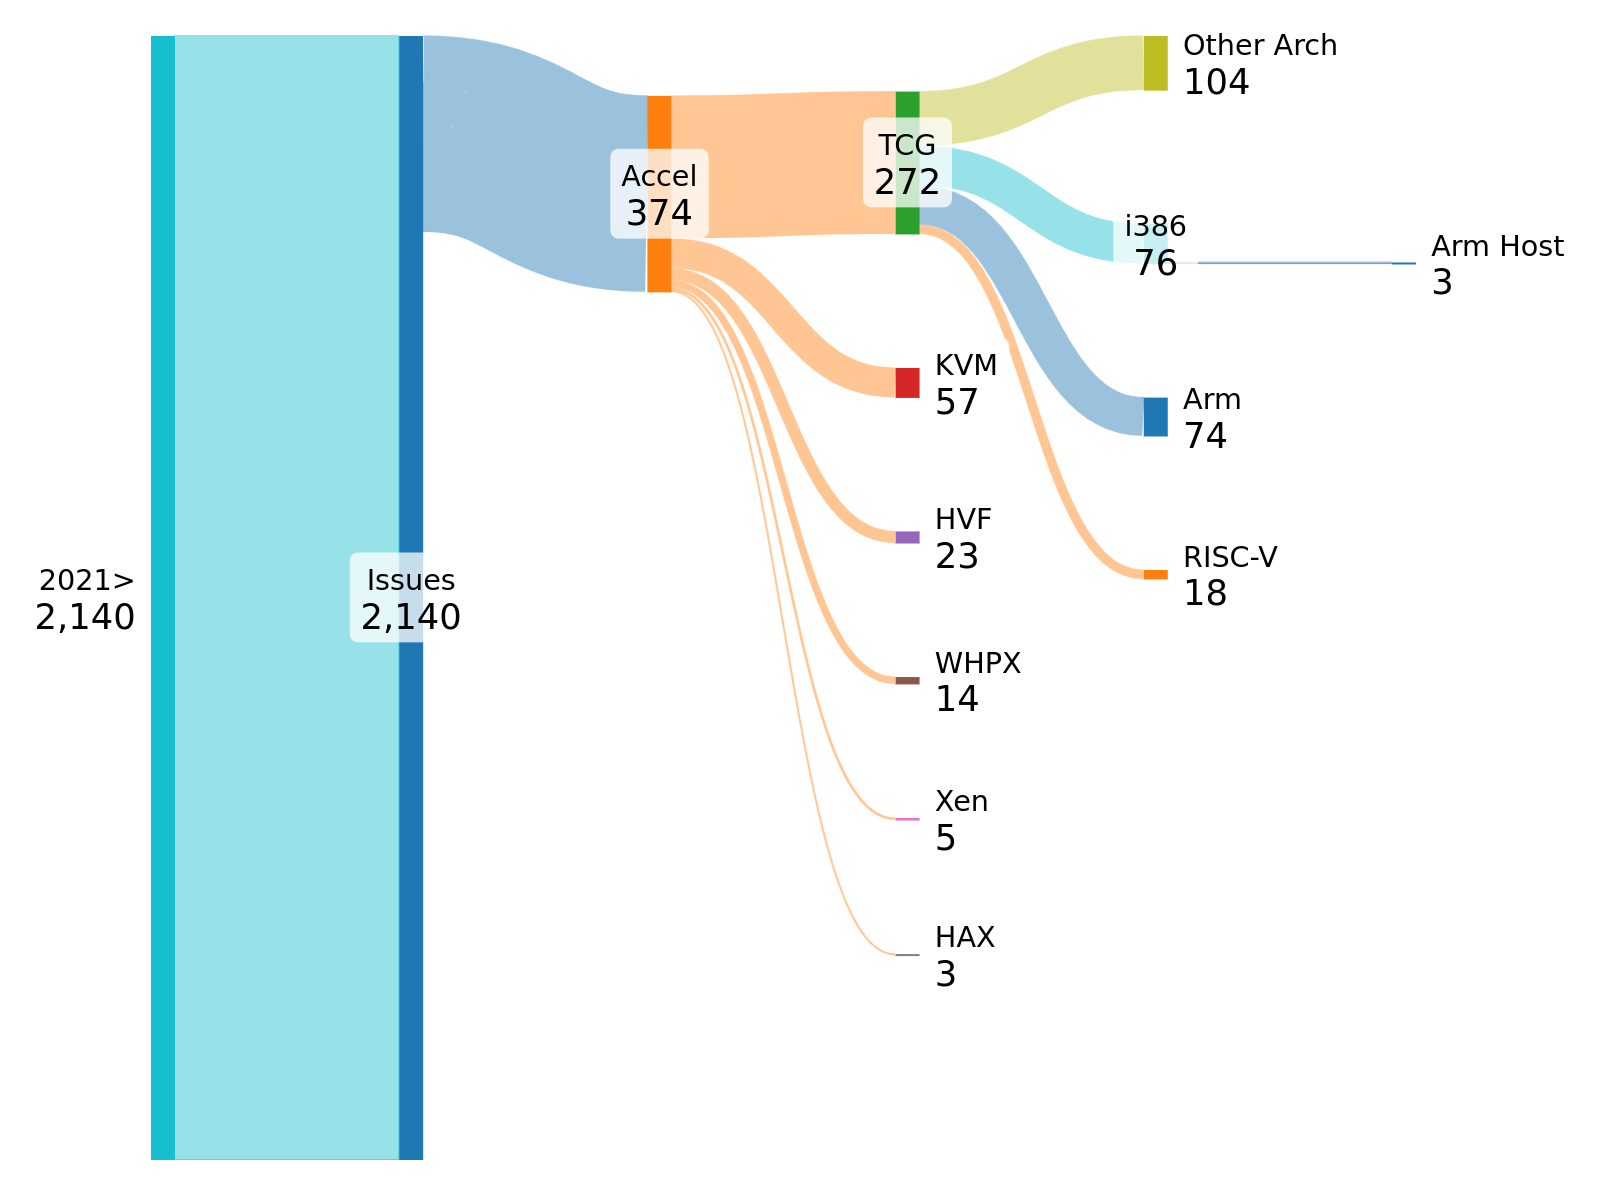
\includegraphics[width=0.8\linewidth]{figures/issues3}
    \caption[QEMU bug distribution]{Sankey diagram showing the distribution of relevant issues}
    \label{fig:issues}
\end{figure}

\section{Distribution of Bugs in QEMU}
As is visible in figure \ref{fig:issues} \ac{QEMU} has more than 2000 bugs.
The current version of \ac{QEMU} is 2038147 \ac{sloc}.
Drawing from Steve McConnell's research on software metrics \cite{sloc}, we can compare QEMU's bug frequency to that of commercially released products, indicating that QEMU has a relatively clean codebase.

Out of all the bugs, 374 are related to accelerators, accounting for about 15\% of the total.
This suggests that accelerator related issues are a significant part of bugs.
Among these accelarator bugs, the majority, or about 70\%, stem from TCG, which is expected given that TCG is the primary and most widely used accelerator.
KVM related bugs make up another 15\%, with the remaining 15\% spread across other areas.

Regarding TCG specific bugs, those involving x86 (i386) and Arm architectures are the most common, each being roughly around 30\% of the total.
This should not come as a surprise since these architectures are being utilized most commonly, leading to extensive usage and testing.

\section{x86 Translation Errors}
In this section, we will go over the bugs encountered when running x86 binaries using the TCG.
Most of these bugs are host architecture and operating system independent and tend to arise from incorrect implementation of individual instructions.

We've organized these bugs into six categories based on how they affect the emulation:
\begin{itemize}
    \item Calculation Error: These are mistakes in instructions that either lead to incorrect calculations or issues with flag registers either being incorrectly set or not set at all. However, they don't usually interrupt the flow of the program.
    \item Exceptions: These bugs trigger an exception in QEMU, causing the emulation to stop abruptly.
    \item Errors: Similar to exceptions, these issues cause QEMU to halt the emulation process.
    \item Segmentation Faults: These occur when the program attempts to access memory areas it doesn't have permission for. While this doesn't happen on actual hardware, it is somehow triggered during the emulation.
    \item Hardware Problems: These bugs impact external hardware, potentially making it unusable or significantly less efficient.
    \item Other Bugs: This category includes bugs that don't fit into the other groups, either because their origin is unclear or because they were introduced in newer versions by mistake.
\end{itemize}

The results of the survey are expressed in the table \ref{tab:tcg_x86}.
In the next sections we will mainly focus on calculation errors, since this is where the verifier shines the most.
It would be challenging to test the other bugs since they don't necessarily finish their execution normaly, therefore leaving the emulator logs incomplete.

\begin{table}[htpb]
    \caption[x86 TCG error distribution]{Distribution of TCG errors for x86.}\label{tab:tcg_x86}
    \centering
    \begin{tabular}{l r r r}
      \toprule
        Type & Number & Closed & Open \\
      \midrule
        Calculation Error & 18 & 12 & 6 \\
        Exceptions & 6 & 4 & 2 \\
        Errors & 3 & 2 & 1 \\
        Segmentation Faults & 14 & 10 & 4 \\
        Hardware Problems & 1 & 0 & 1 \\
        Other & 33 & 26 & 7 \\
      \bottomrule
    \end{tabular}
\end{table}

\subsection{Interpretation and Evaluation of the Bug Survey}
As is visible in table \ref{tcg_x86} most errors in x86 emulation belong to the other category.
These hard to classify bugs, make up nearly 45\% of the total.
Since these errors are complex, is ti quite difficult to test and reproduce them.
Making our project a bad match against them.

There's only a single reported hardware problem, and due to limited information, it's hard to analyse it.
Considering that it is a hardware problem it might not have anything to do with emulated instructions.

Segmentation faults are another frequent issue, accounting for 20\% of all bugs.
These are typically caused by incorrect read and write operations.
Generally the best way to solve these bugs is to trace them and find the location where a read or write causes the segmentation fault.
Even though in case of a segmentation fault the emulator trace will be cut off, considering that we only need to find address where this happens the verifier can be helpful.
However when the reproducer is run it allocates space in the data section.
This means it doesnt consider the cases where some addresses might have special meanings.
For example writing outside the boundaries will be seen as a regular write and will be handled as such, making it difficult to reproduce the bugs accurately.
In these cases the reproducer isn't very helpful.

Errors and exceptions are relatively common in QEMU, leading to the program stopping. These issues likely stem from the emulator's internal state, suggesting that alternative debugging methods might be more effective.

Finally we have the calculation errors.
They make up slightly less than 25\% of total errors but they are theoretically the most challenging to detect as they involve instructions behaving slightly differently than expected.
For example some instruction might set a bit to a wrong value or change another bit that it shouldn't touch.
The main problem with these instructions are that these values are not necessarily used.
Which means these programs can go a long way before exhibiting the bug since the difference might have happened multiple instructions ago.
Or maybe the result is close enough to the expected answer, and therefore is not found out.
However in a good case this instruction just calculates wrong values, and this discrepancy is detected.
Our verifier and reproducer combination is a good match for these instructions since it using symbolic execution we can catch every detail and compare it with the emulator log.

\subsection{Detailed Inspection of Bugs on Arm}
In the following subsections we will go over specific bugs that only appear on arm devices.
We are inspecting these bugs extra throughly because we are interested in seeing whether some bugs appear depending on the host hardware.
Out of 76 bugs that we have seen so far, only 3 of them are Arm specific.
Considering this fact we can assume that hardware specific bugs are rather rare.

\subsubsection{Issue \#1659}
The first issue specific to Arm was discovered in an aarch64 system running Darwin.
This bug caused the emulator to freeze and enter a continuous shutdown loop.
It was traced back to the floatx80\_div instruction.
Upon closer examination, it was determined that the problem was due to a miscompilation by Clang.

Therefore, this issue is not directly related to the emulator itself but to the compiler, meaning we can cross this issue from the Arm only list.

\subsubsection{Issue \#2101}
The second issue was identified on a system using Fedora Linux as the host.
This bug manifests itself when executing the ls command within QEMU.
It results in incorrect output that omits several directories.
Due to the lack of more information, it is not possible to find the actual cause.

\subsubsection{Issue \#2168}
The final issue also happens in Linux.
This time when running grep on Gentoo Linux inside QEMU, a segmentation fault occurs.
Similar to the previous issue, there is limited information available, making it difficult to provide more insights.



